\documentclass[11pt]{article}
\usepackage[T1]{fontenc}
\usepackage[margin=1in]{geometry}
\usepackage{lmodern,microtype,enumitem,booktabs,tabularx,graphicx,xcolor,parskip}
\usepackage[hidelinks]{hyperref}
\definecolor{cherry}{HTML}{BA0C2F}
\newif\ifshowguidance
\showguidancefalse
\newcommand{\guidance}[2]{\ifshowguidance{\small\itshape\color{gray}Suggested length: #1. #2}\par\fi}
\setlist[itemize]{leftmargin=*,itemsep=2pt,topsep=3pt}
\newcommand{\simlabel}{\textbf{Simulated example: software validation only.}}
\begin{document}
\begin{center}
{\Large\textbf{CS 585: Computer Networks, Fall 2026}}\\[4pt]
{\Large\textbf{Final Project Report: Working Draft}}\\[8pt]
{\LARGE\color{cherry}\textbf{Protecting Tail Latency Under Contention}}\\[5pt]
A feasibility study of Linux queue management for mixed workloads\\[8pt]
Draft: November 21, 2026. Final report due December 8, 11:59pm.
\end{center}

\textbf{Evidence status.} We have completed software tests and a preliminary
Linux namespace pilot. The figures labeled simulated come from our toy model.
We have not yet collected the NucBox and MacBook experiment. This draft keeps
those evidence types separate and identifies what the physical run must resolve.

\section*{Team members}
\begin{itemize}
\item Saif Ryan Gangaram, Ph.D. student, Computer Science
\item Jonathan Lloyd, Computer Science
\item Christopher Ong, Computer Science
\item Alejandro Magana Guillen, Computer Science
\end{itemize}

\section{Introduction and motivation}
Our question is whether Linux queue management can protect a small
request-response flow when bulk TCP traffic competes for the same bottleneck.
We compare FIFO, FQ-CoDel, CAKE best-effort, and CAKE with bounded classification.
The goal is to reduce added foreground p99 latency by at least 50\% relative
to FIFO while retaining at least 90\% of FIFO's background goodput.
These thresholds are our feasibility criteria, not established results.

We proposed a three-node Linux testbed, repeated randomized trials, and a
comparison of latency against throughput. Hardware availability changed the
endpoint plan: we now intend to use two MacBooks with a Linux NucBox router.
We also developed a namespace path for controlled software checks and a local
simulation for exercising the analysis. These paths answer different questions.
The physical experiment will test the available equipment; the simulation
cannot tell us which Linux queue policy performs best.

Our preliminary namespace pilot gives a reason to evaluate both goals together.
FQ-CoDel and both CAKE configurations had much lower observed added p99 than
FIFO. Both CAKE variants also retained less than 90\% of FIFO goodput. With only
two paired blocks, generator omissions and unresolved timing checks, we treat
this as a diagnostic result that guides the next experiment.

On November 26 we also ran the workload on this Mac through loopback and
integrated Chris's RPC implementation into the trial runner. The foreground
phase retained 20,000 scheduled slots, including 53 that were not sent. All
20,000 calls in the separate RPC phases completed. This checks the local
collection path while leaving the physical queue-policy question open.

\section{Related work}
Persistent queues can make a busy link feel slow even when its throughput
looks healthy. Gettys and Nichols describe this bufferbloat problem and why
large buffers can hurt interactive traffic~\cite{bufferbloat}. Floyd and
Jacobson's RED work established the value of responding to congestion before
a queue overflows~\cite{red}. Nichols and Jacobson's CoDel instead uses packet
sojourn time to distinguish a standing queue from a transient burst~\cite{codel}.
These studies motivate our latency measurements and unloaded baselines.
We evaluate the deployed FQ-CoDel combination, rather than claiming to isolate
CoDel's contribution from flow scheduling.

Buffer size and traffic aggregation also matter. Appenzeller, Keslassy and
McKeown study how flow multiplexing changes router-buffer requirements~\cite{buffers}.
Their backbone assumptions do not map directly to our small testbed, but they
explain why the number of competing flows belongs in the design. We plan one
and eight background flows while holding aggregate offered demand fixed.

CAKE is the closest prior system to our experiment. H{\o}iland-J{\o}rgensen,
T{\"a}ht and Morton combine shaping, queue management and traffic isolation
for home gateways~\cite{cake}. We compare its best-effort mode with a bounded
classification rule for our foreground replies. The classification budget
matters because a priority policy that starves bulk traffic would fail our
goodput criterion. Our workload and repeatability checks are a small feasibility
study of these existing mechanisms, not a new queue-management algorithm.

DCTCP examines small foreground work competing with large transfers in data
centers~\cite{dctcp}. It changes endpoint congestion control using ECN, whereas
our main treatments change the Linux router. Dean and Barroso explain why
occasional slow responses can dominate a distributed service's user-visible
latency~\cite{tail}. Together, these papers support looking beyond averages,
but neither makes our 512-byte request stream a validated model of a complete
production service.

Finally, Flent shows why repeated network experiments need coordinated traffic,
metadata and reproducible analysis~\cite{flent}. Our collector follows that
measurement concern with retained attempts, hashes and explicit request
accounting. We use a custom foreground program and iperf3 rather than claiming
that our current pipeline runs Flent. Its methodology remains a useful
independent cross-check for the final study.

\section{Technical implementation}
\subsection{Topology and treatments}
The intended physical path is client MacBook, Linux NucBox router, then server
MacBook, with dedicated wired links and separate Wi-Fi management. The client
uses 10.203.0.2/30 and the server uses 10.203.0.6/30. Each has an explicit host
route to its peer through the router. Our preflight refuses a selected Mac
default-route interface, incorrect address or mask, or mismatched source revision.
Each workload also requires an active Ethernet link after router setup.
The Mac helpers inspect existing network settings
without changing them. The Linux helper owns a private router namespace and
temporarily attaches only the two explicitly selected, unused Ethernet ports.

The shaped return path is 100 Mb/s. FIFO uses a 250,000-byte queue below HTB;
FQ-CoDel uses the same shaper with its own queue. The CAKE treatments shape
directly at 100 Mb/s. The bounded variant classifies only the designated
foreground reply flow and applies a 5 Mb/s policing budget. Incoming DS fields
are cleared before our own classification. These are documented candidate
settings that still need team acceptance on the final hardware.

In the mixed topology, NetEm adds 20 ms on router egress toward the server.
The Linux-only topology instead adds 10 ms on each endpoint's ingress.
Both target about 20 ms of added base RTT, but the queue placement differs.
We record the mixed topology separately and do not pool its results with the
namespace or all-Linux physical runs. The Mac endpoints retain native TCP
behavior. Linux TCP\_INFO and AF\_PACKET measurements are unavailable there.

\subsection{Workloads and lifecycle}
The candidate foreground workload sends 512-byte messages at 500 requests per
second using the client's monotonic clock. UDP is the main planned transport;
TCP is a separately labeled sensitivity experiment with fixed framing and
TCP\_NODELAY. Reverse TCP iperf3 traffic supplies background demand at 50\%,
90\% or 110\% of the shaped rate, split across one or eight flows. Offered
demand above capacity does not imply delivered throughput above capacity.

The pilot has two blocks, four policies, unloaded baselines and a 110 Mb/s
single-flow condition: 16 trials. The larger plan has ten 60-second trials
for each loaded condition and ten unloaded trials per policy: 280 trials.
Policy order is randomized within recorded blocks. Physical collection is
serial because simultaneous trials would share the bottleneck and invalidate
the comparison. Local simulation uses up to eight worker processes; its
default six blocks produce 48 trials and 240,000 scheduled slots, three times
the pilot volume.

Each trial records its source, configuration, lifecycle, observations and
artifact hashes in a fresh directory. Failed attempts remain available.
Commands have deadlines and bounded output. Cancellation stops owned child
processes and preserves cleanup errors. Endpoint leases prevent overlapping
trials. Linux cleanup verifies resource identity before returning interfaces.
The pipeline proceeds automatically from successful collection to checked
export, analysis, plots and a text interpretation.

\subsection{Analysis and verification}
We calculate per-run latency percentiles and match loaded runs to their
unloaded baseline in the same block. Added p99 is loaded p99 minus unloaded
p99. Policy comparisons use paired block resampling for 95\% bootstrap
intervals; individual requests are not independent replications. The pipeline
retains generator omissions, timeouts and late replies. A low on-time p99
without those outcomes can be misleading.

Our exploratory analysis standardizes six run metrics and fits K-means, Ward
agglomerative clustering and DBSCAN. PCA and t-SNE display those metrics;
t-SNE itself is not a clustering algorithm. Noise points remain in all
comparisons. Ridge and Lasso use design features with entire blocks held out;
scaling and penalty selection use only training folds. At least six blocks
are required. These models describe observed designs and do not establish
causality or transfer to new hardware.

Jonathan's original comparison workflow and Chris's C++ networking prototype
remain in the repository with their authorship intact. The C++ probe is a
separate workload check, not the source of the main foreground metric. Our
unit and integration checks cover data validation, real sockets, subprocess
failures and cleanup. CI enforces 95\% statement and branch coverage separately
for core and analysis, with a separate Linux job for privileged testbed checks.
Hardware acceptance remains a separate activity.

For $N$ requests, per-run sorting costs $O(N\log N)$ time and $O(N)$ auxiliary
memory. Analysis bounds each export batch at 200,000 request rows and keeps
at most 400 run summaries for the offline models. Ward and DBSCAN can require
$O(R^2)$ work or storage for $R$ runs; the fixed run cap bounds that cost.
Foreground accounting bounds active requests at 1,024. Ruff enforces McCabe
complexity at most 10 per function. These limits support review and predictable
failure behavior; coverage and complexity scores do not certify correctness.

\section{Cost analysis}
Our proposal budget was \$330: \$220 for a dual-port mini PC, \$80 for two
USB-C Ethernet adapters, and \$30 for three cables. These remain planning
estimates, not verified receipts. We have the NucBox and previously reported
adapters and cables, but the final Mac connections and compatibility still
need confirmation. We will add actual expenses and borrowed-equipment details
after setup rather than treat the estimate as money spent.

The two MacBooks are existing equipment. The software has no project-specific
license purchase, but installation, verification, troubleshooting and analysis
take time. The 280-run design alone contains 16,800 measured seconds, or
4 hours 40 minutes, plus warmup, per-trial setup, cleanup and checks. A repeat
or sensitivity study adds to that commitment. We have not kept a verified
person-hour ledger, so this draft does not invent a labor total.

The local model reduces software-check turnaround. In the repository's recorded
three-repeat benchmark, four workers had a median collection time of 0.273 s
versus 0.822 s for one worker, about 3.01 times faster, for the same 240,000
slots. This measures toy-data collection only. It does not shorten the required
physical observation windows or establish a general multiprocessing speedup.

\section{Community analysis}
The immediate audience is students and small-network operators who need to
understand why a fast bulk transfer can coexist with poor interactive response.
The bufferbloat and CAKE literature documents this problem in access networks
and motivates evaluating latency alongside throughput~\cite{bufferbloat,cake}.
Our contribution is a small reproducible comparison with visible measurement
limits, rather than a claim that we have identified a universal best policy.

A useful result would help someone decide what to measure before changing a
gateway: unloaded latency, contention behavior, delivered goodput and failures.
We have not interviewed users or measured a campus or household deployment.
Our conclusions will therefore apply to the tested workload and equipment.
Wi-Fi contention, multiple households, encrypted application classification
and fairness between real users remain outside this experiment.

Bounded priority also has a community consequence. Improving one selected
flow can reduce service for others. We retain bulk goodput in the success
criteria and keep the unfavorable CAKE pilot results visible. Before proposing
deployment, we would need stronger fairness and abuse checks and evidence
from representative traffic.

\section{Findings}
\subsection{Simulated analysis example}
\simlabel{} The current example has six blocks, 48 trials and 240,000 scheduled
slots. Its policy factors are assumptions built into the model. Table~\ref{tab:sim}
shows the 110 Mb/s, one-flow condition. The results demonstrate the reporting
path; they do not validate Linux queue behavior.

\begin{table}[htbp]\centering
\caption{Simulated example. Six paired blocks per policy.}\label{tab:sim}
\begin{tabular}{lrr}\toprule
Policy & Added on-time p99 (ms) & FIFO goodput retained (\%)\\\midrule
FIFO & 15.942 & 100.00\\
FQ-CoDel & 4.769 & 98.75\\
CAKE best-effort & 3.228 & 94.31\\
CAKE bounded & 2.550 & 95.77\\\bottomrule
\end{tabular}
\end{table}

The model includes 967 unsent slots and 108 timeout or late outcomes. Its
K-means and Ward fits have silhouette 0.212; DBSCAN finds one dense group and
labels 19 of the 24 loaded runs as noise. This disagreement is a useful warning
against treating a two-dimensional cluster picture as proof of distinct network
regimes. We keep every run. Ridge and Lasso have held-out-block MAE of 0.0358
and 0.0426 ms, respectively, compared with 4.659 ms for the training-mean
baseline. The small errors reflect a simple, deliberately structured toy
generator. They are not evidence of prediction accuracy on real traffic.

\begin{figure}[htbp]\centering
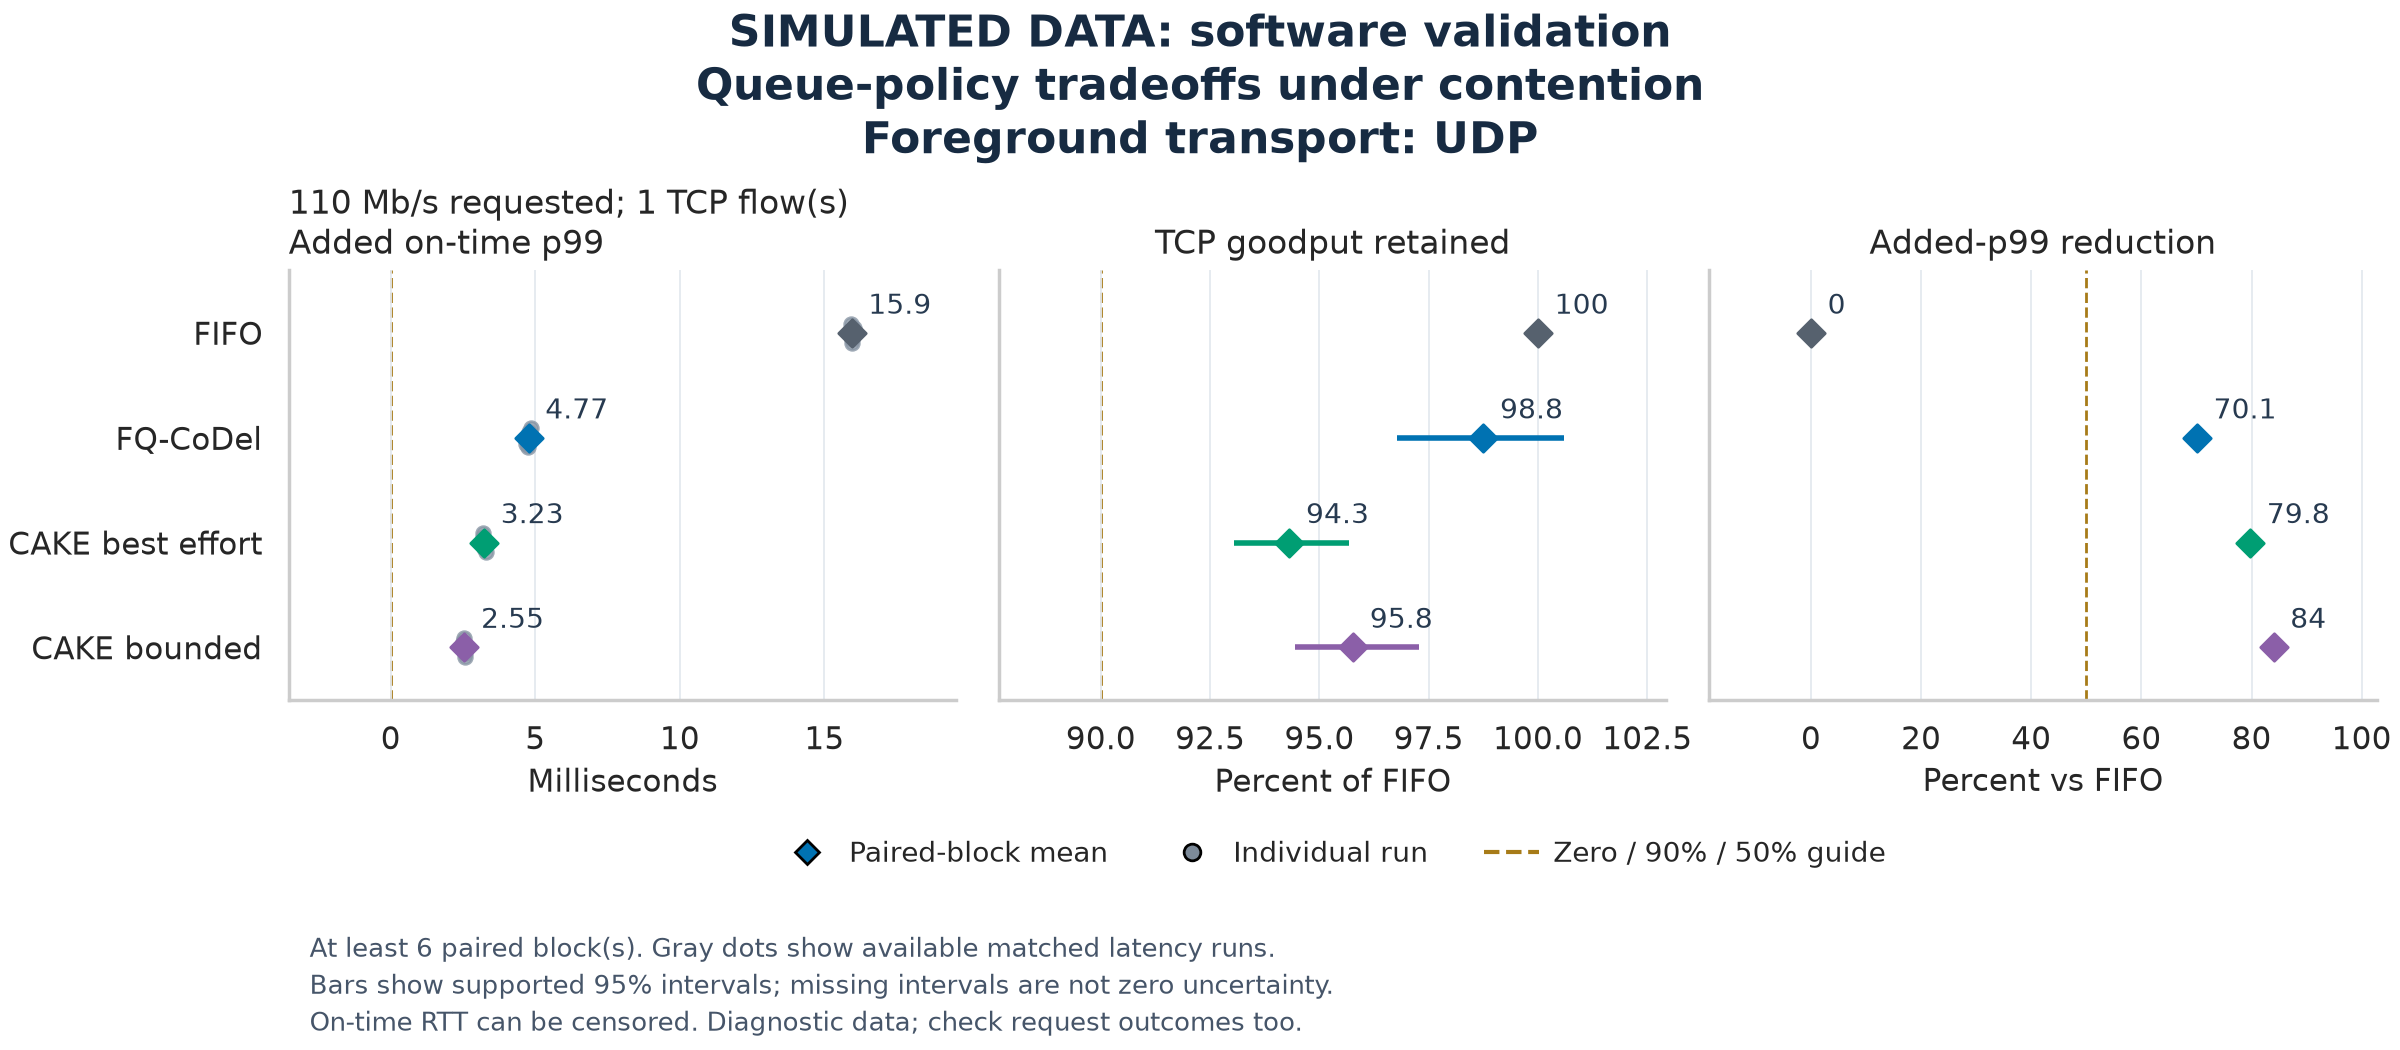
\includegraphics[width=\linewidth]{../analysis/plots/simulation/policy_comparisons.png}
\caption{Simulated policy comparison from the recorded six-block example.
Intervals describe variation in the toy model, not uncertainty about hardware.}
\end{figure}

\subsection{Existing namespace measurements}
The separate November 11 namespace pilot contains 16 completed trials and
80,000 scheduled measurement slots. It retained 3,192 unsent slots (3.99\%),
with no recorded timeout or late outcomes. Table~\ref{tab:pilot} reports the
two-block means. The analysis withholds confidence intervals because there
are too few blocks. The source is the retained e3ddaff export from hosted
Linux workflow 43111991762, available in the repository's reference directory.

\begin{table}[htbp]\centering
\caption{Observed namespace pilot, two paired blocks. No physical NucBox measurements.}\label{tab:pilot}
\begin{tabular}{lrr}\toprule
Policy & Added on-time p99 (ms) & FIFO goodput retained (\%)\\\midrule
FIFO & 18.977 & 100.00\\
FQ-CoDel & 0.104 & 99.37\\
CAKE best-effort & 0.106 & 89.37\\
CAKE bounded & 0.094 & 89.18\\\bottomrule
\end{tabular}
\end{table}

Both CAKE variants miss the 90\% goodput target in this pilot despite the
lower observed on-time p99. FQ-CoDel meets both point-estimate targets here,
but the small sample, omitted sends and shared-host environment prevent a
strong recommendation. We cannot infer that a missing request would have
experienced the same latency as a request that was sent.

\subsection{What the physical run must establish}
The NucBox/MacBook run must first establish the actual link path, base RTT,
queue attachment, offered and achieved load, and generator behavior. We will
replace the simulated comparison with the measured per-condition results,
paired intervals and outcome counts while retaining the reference example
separately. A treatment will count as feasible only if both stated targets
are supported by valid evidence, with uncertainty reported.

Exact foreground and bulk measurement-window alignment remains unresolved.
The retained iperf3 receiver interval is checked against its byte totals but
does not prove alignment with the foreground window. Router CPU is also
unavailable in the mixed endpoint collector. Native Mac TCP behavior, USB
adapter effects and the changed delay placement limit comparison with the
Linux-only pilot. We will report these limitations and any failed runs rather
than turn successful pipeline execution into a scientific success claim.

\section{Conclusion and next steps}
We have a repeatable software path for collecting, checking and analyzing the
queue-policy experiment, with a separate macOS endpoint configuration for the
equipment now available. The simulated example exercises that path. The
namespace pilot suggests a substantial latency difference under contention,
but it also shows why our conclusion needs both latency and goodput: both
CAKE variants missed the proposed throughput-retention target.

Our strongest current lesson concerns measurement. A low on-time percentile
can coexist with unsent requests, and a favorable latency result can coexist
with an unfavorable goodput result. We need those quantities together before
deciding whether a policy helped.

Next we will verify the Ethernet setup, run the physical pilot, inspect its
quality checks and agree on the remaining protocol choices. We will then
collect the larger design if the pilot supports it, update the figures and
conclusions, and rehearse the four-person presentation. The open question for
the class is how much throughput loss is acceptable for interactive traffic
and what workload would make that tradeoff meaningful. The final report is
due December 8; no physical result is claimed in this working draft.

\bibliographystyle{IEEEtran}
\bibliography{references}
\end{document}
